% Numeric source: paper/shared/evidence/raw/iclr_model_behavior/analysis_v1/results.json
\section{Navigation: Small Net Changes, Different Successful Episodes}
\label{sec:navigation}

The downstream experiment asks what happens when a language-conditioned agent
observes converted scenes throughout an episode. We evaluate InternNav/DualVLN
on the three KuJiaLe scenes in the official \texttt{val\_unseen} package used here,
with 33 episodes per scene. The paired run comprises \NavN\ episode pairs and
198 rollouts. Both conditions use the same episode IDs and task definitions.
The agent receives each material condition throughout closed-loop execution.

\begin{table}[t]
\centering\small
% Generated by scripts/build_assets.py from corrected results.json
\begin{tabular}{lrrrrrr}
\toprule
Scene & $N$ & $SR_O$ & $SR_C$ & $SPL_O$ & $SPL_C$ & Flips \\
\midrule
0031 & 33 & 51.5 & 57.6 & 47.9 & 49.6 & 8 \\
0036 & 33 & 81.8 & 60.6 & 70.0 & 55.0 & 11 \\
0066 & 33 & 24.2 & 27.3 & 24.2 & 24.3 & 11 \\
\midrule
All & 99 & 52.5 & 48.5 & 47.4 & 43.0 & 30 \\
\bottomrule
\end{tabular}

\caption{Paired navigation results by scene. SR and SPL are percentages;
O and C denote original and converted materials. Flips count episodes whose
success status changes between conditions.}
\label{tab:navigation}
\end{table}

\paragraph{Outcome cancellation hides decision turnover.}
Across the \NavN\ pairs, original materials yield 52 successful episodes and
converted materials yield 48. The net loss of four consists of 17
success-to-failure transitions and 13 failure-to-success transitions.
Consequently, \NavFlips\ of \NavN\ episodes change success status:
\NavFlipPercent\% turnover despite a 4.0 percentage-point aggregate SR change.
Figure~\ref{fig:navigation} exposes this cancellation directly. An unchanged
mean would not imply that the same instructions still succeed.

\begin{figure}[t]
\centering
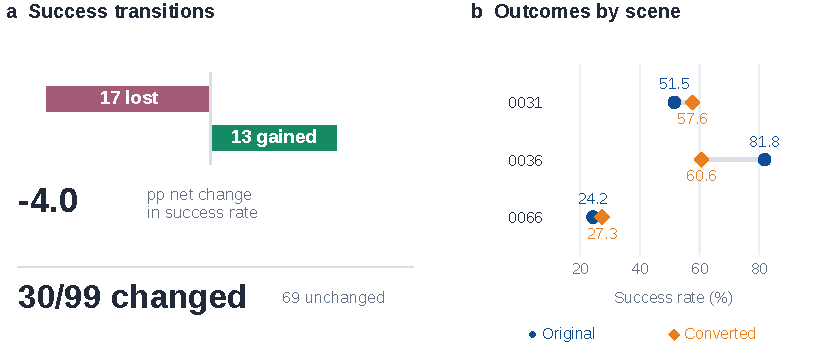
\includegraphics[width=\linewidth]{navigation.pdf}
\caption{Paired navigation outcomes. Left: 17 losses and 13 gains produce
30 changes but a small net decrease. Right: scene-level success rates reveal
opposing effects. The remaining 69 pairs retain their outcome.}
\label{fig:navigation}
\end{figure}

\paragraph{Scene dependence.}
Scene 0036 contributes the largest net decrease, from 81.8\% to 60.6\% success,
while scenes 0031 and 0066 improve in aggregate. SPL follows the largest
decrease in scene 0036. Across all scenes, mean NE changes from 3.680 to 3.631,
while mean TL changes from 6.975 to 7.060. These summaries describe different
aspects of the trajectory: endpoint error, path efficiency, and binary completion
need not move together. Retaining the episode-level transitions makes those
differences visible instead of compressing them into a single stability score.

\paragraph{From outcomes to paths.}
Figure~\ref{fig:trajectories} pairs ending observations with map excerpts from
recorded reruns of three episode IDs. The views show how the agent's surroundings
and path differ across material conditions. Appendix~\ref{app:navigation}
expands these comparisons to twelve recorded episode pairs.

\begin{figure}[!t]
\centering
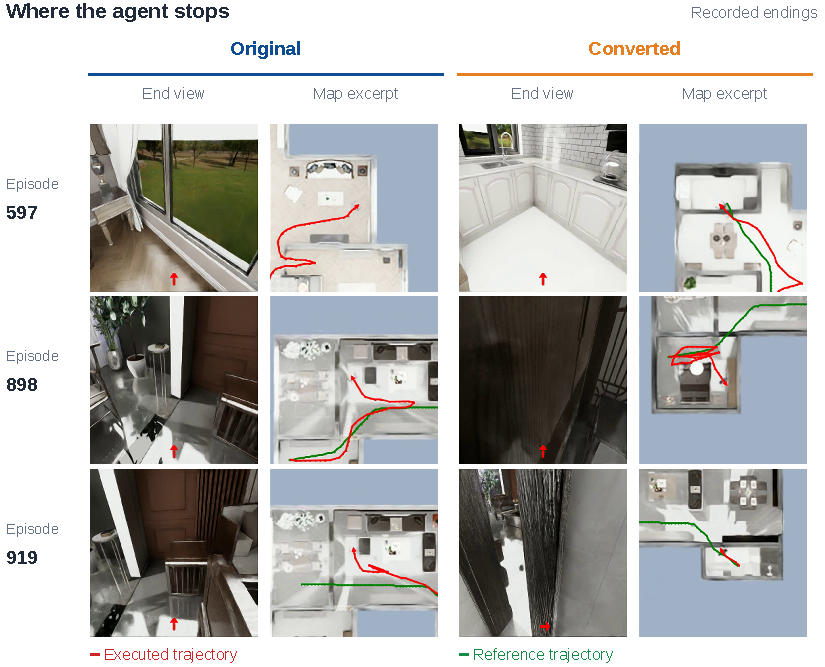
\includegraphics[width=\linewidth]{trajectories.pdf}
\caption{Recorded ending views and map excerpts from separate qualitative
reruns. Red view symbols indicate actions; red and green map lines show executed
and reference paths. Table~\ref{tab:navigation} reports the separate 99-pair metric runs.}
\label{fig:trajectories}
\end{figure}
